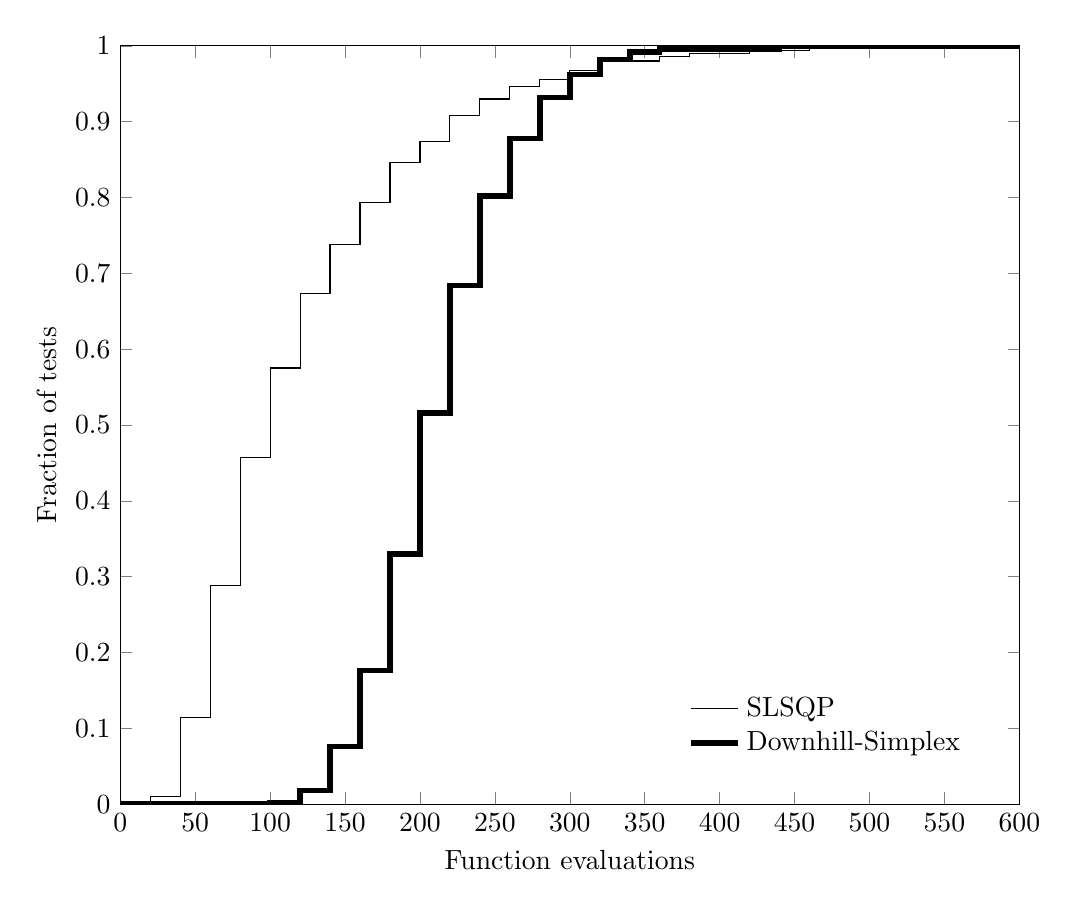
\begin{tikzpicture}
  \begin{axis}[
    width=13cm,
    ylabel=Fraction of tests,
    xlabel=Function evaluations,
    xmin=0,xmax=600,ymin=0,ymax=1,
    legend style={
      draw=none,
      at={(0.95,0.05)},
      anchor=south east,
      cells={anchor=west}}]
    \addplot [const plot] coordinates {
(0.00000000e+00, 0.00000000e+00)
(2.00000000e+01, 1.00200401e-02)
(4.00000000e+01, 1.14228457e-01)
(6.00000000e+01, 2.88577154e-01)
(8.00000000e+01, 4.56913828e-01)
(1.00000000e+02, 5.75150301e-01)
(1.20000000e+02, 6.73346693e-01)
(1.40000000e+02, 7.37474950e-01)
(1.60000000e+02, 7.93587174e-01)
(1.80000000e+02, 8.45691383e-01)
(2.00000000e+02, 8.73747495e-01)
(2.20000000e+02, 9.07815631e-01)
(2.40000000e+02, 9.29859719e-01)
(2.60000000e+02, 9.45891784e-01)
(2.80000000e+02, 9.55911824e-01)
(3.00000000e+02, 9.67935872e-01)
(3.20000000e+02, 9.79959920e-01)
(3.40000000e+02, 9.79959920e-01)
(3.60000000e+02, 9.85971944e-01)
(3.80000000e+02, 9.89979960e-01)
(4.00000000e+02, 9.89979960e-01)
(4.20000000e+02, 9.93987976e-01)
(4.40000000e+02, 9.93987976e-01)
(4.60000000e+02, 9.95991984e-01)
(4.80000000e+02, 9.95991984e-01)
(5.00000000e+02, 9.97995992e-01)
(5.20000000e+02, 9.97995992e-01)
(5.40000000e+02, 9.97995992e-01)
(5.60000000e+02, 9.97995992e-01)
(5.80000000e+02, 1.00000000e+00)
(6.00000000e+02, 1.00000000e+00)
    };
    \addplot [const plot,line width=2pt] coordinates {
(0.00000000e+00, 0.00000000e+00)
(2.00000000e+01, 0.00000000e+00)
(4.00000000e+01, 0.00000000e+00)
(6.00000000e+01, 0.00000000e+00)
(8.00000000e+01, 0.00000000e+00)
(1.00000000e+02, 2.00000000e-03)
(1.20000000e+02, 1.80000000e-02)
(1.40000000e+02, 7.60000000e-02)
(1.60000000e+02, 1.76000000e-01)
(1.80000000e+02, 3.30000000e-01)
(2.00000000e+02, 5.16000000e-01)
(2.20000000e+02, 6.84000000e-01)
(2.40000000e+02, 8.02000000e-01)
(2.60000000e+02, 8.78000000e-01)
(2.80000000e+02, 9.32000000e-01)
(3.00000000e+02, 9.62000000e-01)
(3.20000000e+02, 9.82000000e-01)
(3.40000000e+02, 9.92000000e-01)
(3.60000000e+02, 9.96000000e-01)
(3.80000000e+02, 9.96000000e-01)
(4.00000000e+02, 9.96000000e-01)
(4.20000000e+02, 9.96000000e-01)
(4.40000000e+02, 1.00000000e+00)
(4.60000000e+02, 1.00000000e+00)
(4.80000000e+02, 1.00000000e+00)
(5.00000000e+02, 1.00000000e+00)
(5.20000000e+02, 1.00000000e+00)
(5.40000000e+02, 1.00000000e+00)
(5.60000000e+02, 1.00000000e+00)
(5.80000000e+02, 1.00000000e+00)
(6.00000000e+02, 1.00000000e+00)    };
    \legend{SLSQP,Downhill-Simplex}
  \end{axis}
\end{tikzpicture}
